\documentclass{article}
\usepackage[margin=1in]{geometry}
\usepackage{graphicx}
\usepackage{booktabs}
\usepackage{float}
\usepackage{amsmath}
\usepackage{amssymb}
\usepackage{hyperref}
\usepackage{subcaption}

\title{IFT6135 - Assignment 3 Report}
\author{Guillaume Genois, 20248507}
\date{April 28, 2026}

\begin{document}

\maketitle

%==============================================================================
\section*{Problem 1: Denoising Diffusion Probabilistic Models}
%==============================================================================

% -----------------------------------------------------------------------------
\subsection*{Question 8: Training progression and sample quality}

\begin{figure}[H]
  \centering
  \begin{subfigure}[t]{0.32\textwidth}
    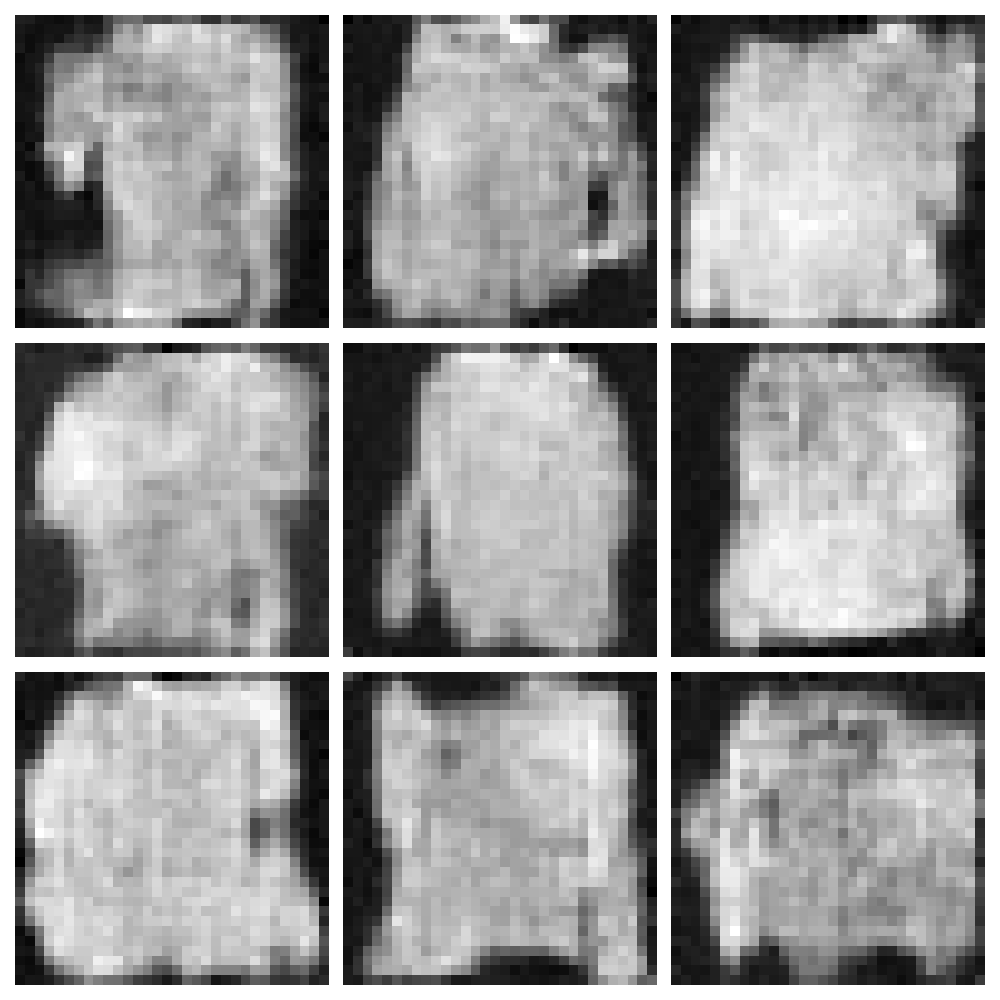
\includegraphics[width=\linewidth]{epoch_2_sample_999.png}
    \caption{Epoch 2}
  \end{subfigure}\hfill
  \begin{subfigure}[t]{0.32\textwidth}
    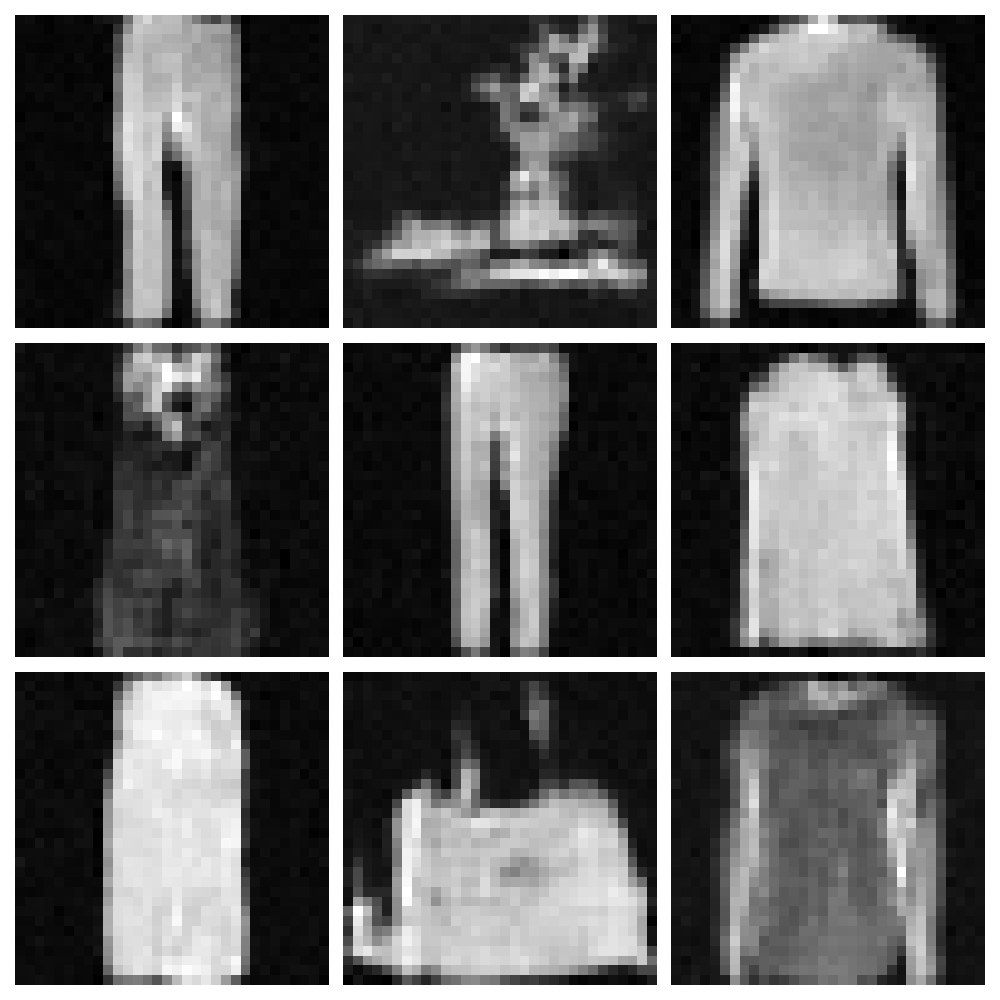
\includegraphics[width=\linewidth]{epoch_10_sample_999.png}
    \caption{Epoch 10}
  \end{subfigure}\hfill
  \begin{subfigure}[t]{0.32\textwidth}
    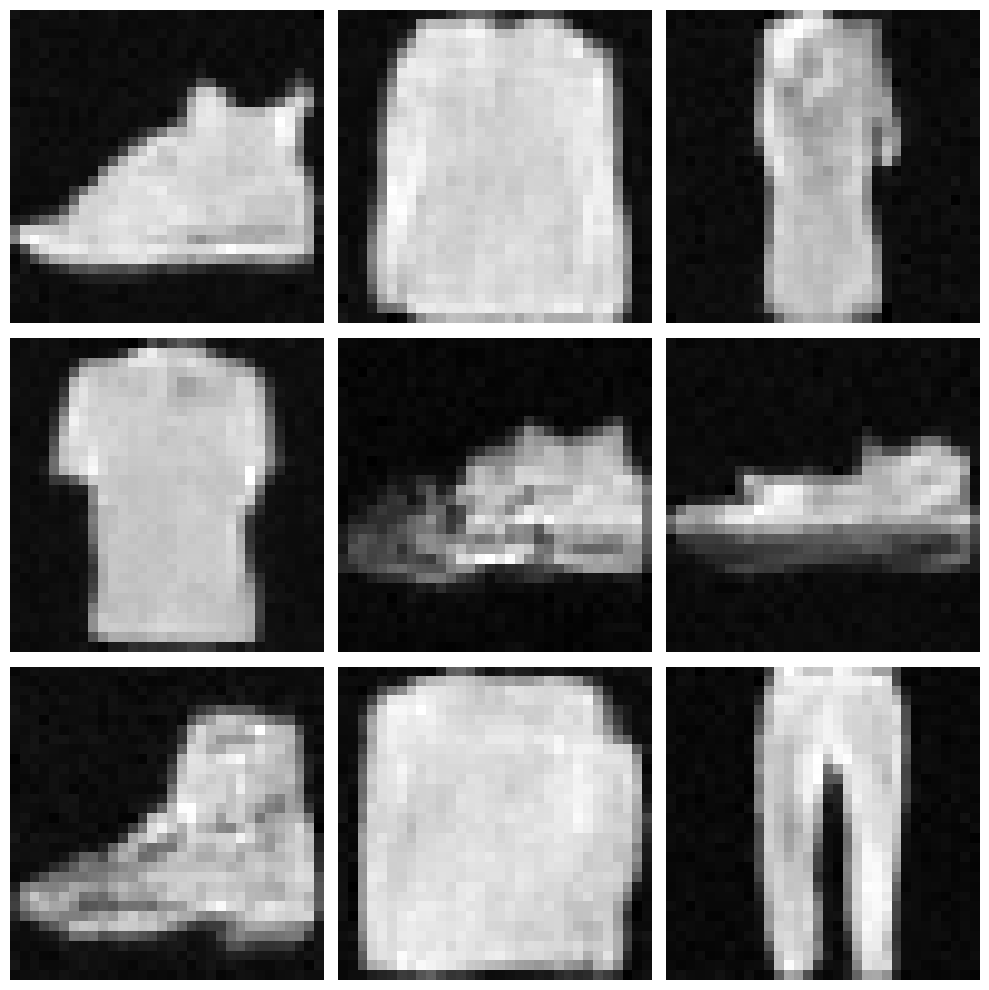
\includegraphics[width=\linewidth]{nb_q1_epoch_18.png}
    \caption{Epoch 18}
  \end{subfigure}
  \caption{DDPM unconditional samples ($3\times 3$ grids at $32\times 32$) drawn
           from the model at three points during training.}
  \label{fig:ddpm_grids}
\end{figure}

\subsubsection*{Sample sharpness}

At epoch-2, the model has only seen the dataset twice and the reverse chain
returns rough rectangular blobs of uniform luminance, with no recognizable
garment structure. After only two epochs, the noise predictor seems to have learned the
marginal pixel statistics and the bulk shape prior (objects on a dark
background, roughly square footprint) but not yet category-specific structure.

By epoch-10, most cells in the grid contain unambiguous FashionMNIST
silhouettes (trousers, long-sleeve top, dress, skirt, knit pullover), with
crisp object and background separation, and only mild blur at the edges. By
epoch-18, edges seem sharper, but many samples are still a bit weird looking with difficulties with sleeves. The differences between epoch-10 and 18 don't seem to be too big.

\subsubsection*{Diversity}

The epoch-18 grid alone covers at least seven of the ten FashionMNIST
categories (sneaker, ankle boot, pullover, t-shirt, trousers, sandal/slipper,
heeled shoe, dress) across nine cells, which suggests the model has not
collapsed to a small subset of modes.

\subsubsection*{Common failure modes}

\begin{itemize}
  \item \textbf{Fractal textures:} A small fraction
    of samples (e.g.\ the top-middle cell at epoch~10) seems to contain noise-like or fractal-looking textures rather than a
    recognizable garment. These look like trajectories that the reverse
    chain failed to commit to any nearby data mode.
  \item \textbf{Residual blur:} Even at epoch-18, large flat regions (the
    body of a sweater, the leg of a trouser) remain perceptibly softer than
    real $32\times 32$ FashionMNIST images. This is the expected price of
    the simplified $L_2$ objective, which regresses against the mean of
    plausible completions.
  \item \textbf{Asymmetric or truncated extremities:} Several cells have
    one sleeve cleanly resolved and the other faded,
    broken, or noticeably thinner (e.g.\ the left sleeve of the
    dress at the top-right of the epoch-18 grid). Where the dataset has
    multiple plausible sleeve completions for a given silhouette,
    the $L_2$ noise predictor seems to average over them and commit to a
    compromise that visibly mismatches the surrounding garment.
\end{itemize}

\subsubsection*{Practical improvements}

\begin{itemize}
  \item \textbf{Cosine $\beta$ schedule:} The linear schedule used here drops
    the signal-to-noise ratio to near zero across most of the chain, so the
    network spends most of its training budget on timesteps where there is
    essentially no signal left to predict. The cosine schedule keeps the signal-to-noise ratio bounded away from zero through more of
    the chain, which could help reduce the residual blur observed
    above by giving the network more useful gradient signal at
    intermediate $t$.
  % \item \textbf{No-noise final step.} Algorithm 2 of Ho et al.\ (2020)
  %   skips the random-noise injection at the very last reverse step, so the
  %   final iterate is exactly the deterministic mean predicted by the
  %   network. The current implementation still injects fresh noise at every
  %   step including the last, which adds a small amount of unnecessary
  %   variance to the final pixel values. The fix is a one-line guard around
  %   the noise sampling, has no effect on the rest of the chain, and is
  %   essentially free.
  % \item \textbf{EMA model at sampling time.} The trainer already maintains
  %   a slowly-updated moving average of the network weights, but the
  %   snapshot callback samples from the live weights. Switching the
  %   callback to the EMA weights averages out high-frequency oscillation in
  %   the optimizer trajectory and is widely reported to improve sample
  %   fidelity at no additional training cost, since the EMA copy is already
  %   resident in GPU memory.
  % \item \textbf{Classifier-free guidance.} FashionMNIST ships with class
  %   labels that the current unconditional model ignores. Training the
  %   U-Net to also predict noise conditioned on the class label, with
  %   occasional random label dropout so the model still learns the
  %   unconditional case, lets the sampler combine the two predictions and
  %   push the trajectory toward the chosen class. This would directly
  %   target the two perceptual failures observed by anchoring the garbled /
  %   fractal cells (which look like trajectories that never committed to a
  %   data mode) to a specific class and shrinking the residual blur. The
  %   usual tradeoff is reduced within-class diversity, so the guidance
  %   strength is a tunable knob.
  \item \textbf{Longer training:} The training loss was still trending
    down at the end of 20 epochs, so simply training for longer should provide additional quality, with no architectural
    change required.
  \item \textbf{Deeper or wider U-Net backbone:} Adding base channels,
    residual blocks per resolution, or self-attention layers at the
    bottleneck would increase the network's capacity to synthesize
    high-frequency texture in the structure-forming regime near $t = 0$,
    which is where most of the perceptual quality is decided.
  \item \textbf{Learned reverse variance:} The current implementation
    fixes $\sigma_t^2 = \beta_t$ at every reverse step. Letting the network also predict $\sigma_\theta(\mathbf{x}_t, t)$
    could improve both negative log-likelihood and sample
    quality, since the optimal reverse variance lies between two natural
    bounds rather than at either endpoint.
\end{itemize}

% -----------------------------------------------------------------------------
\subsection*{Question 9: Intermediate denoising stages}

\begin{figure}[H]
  \centering
  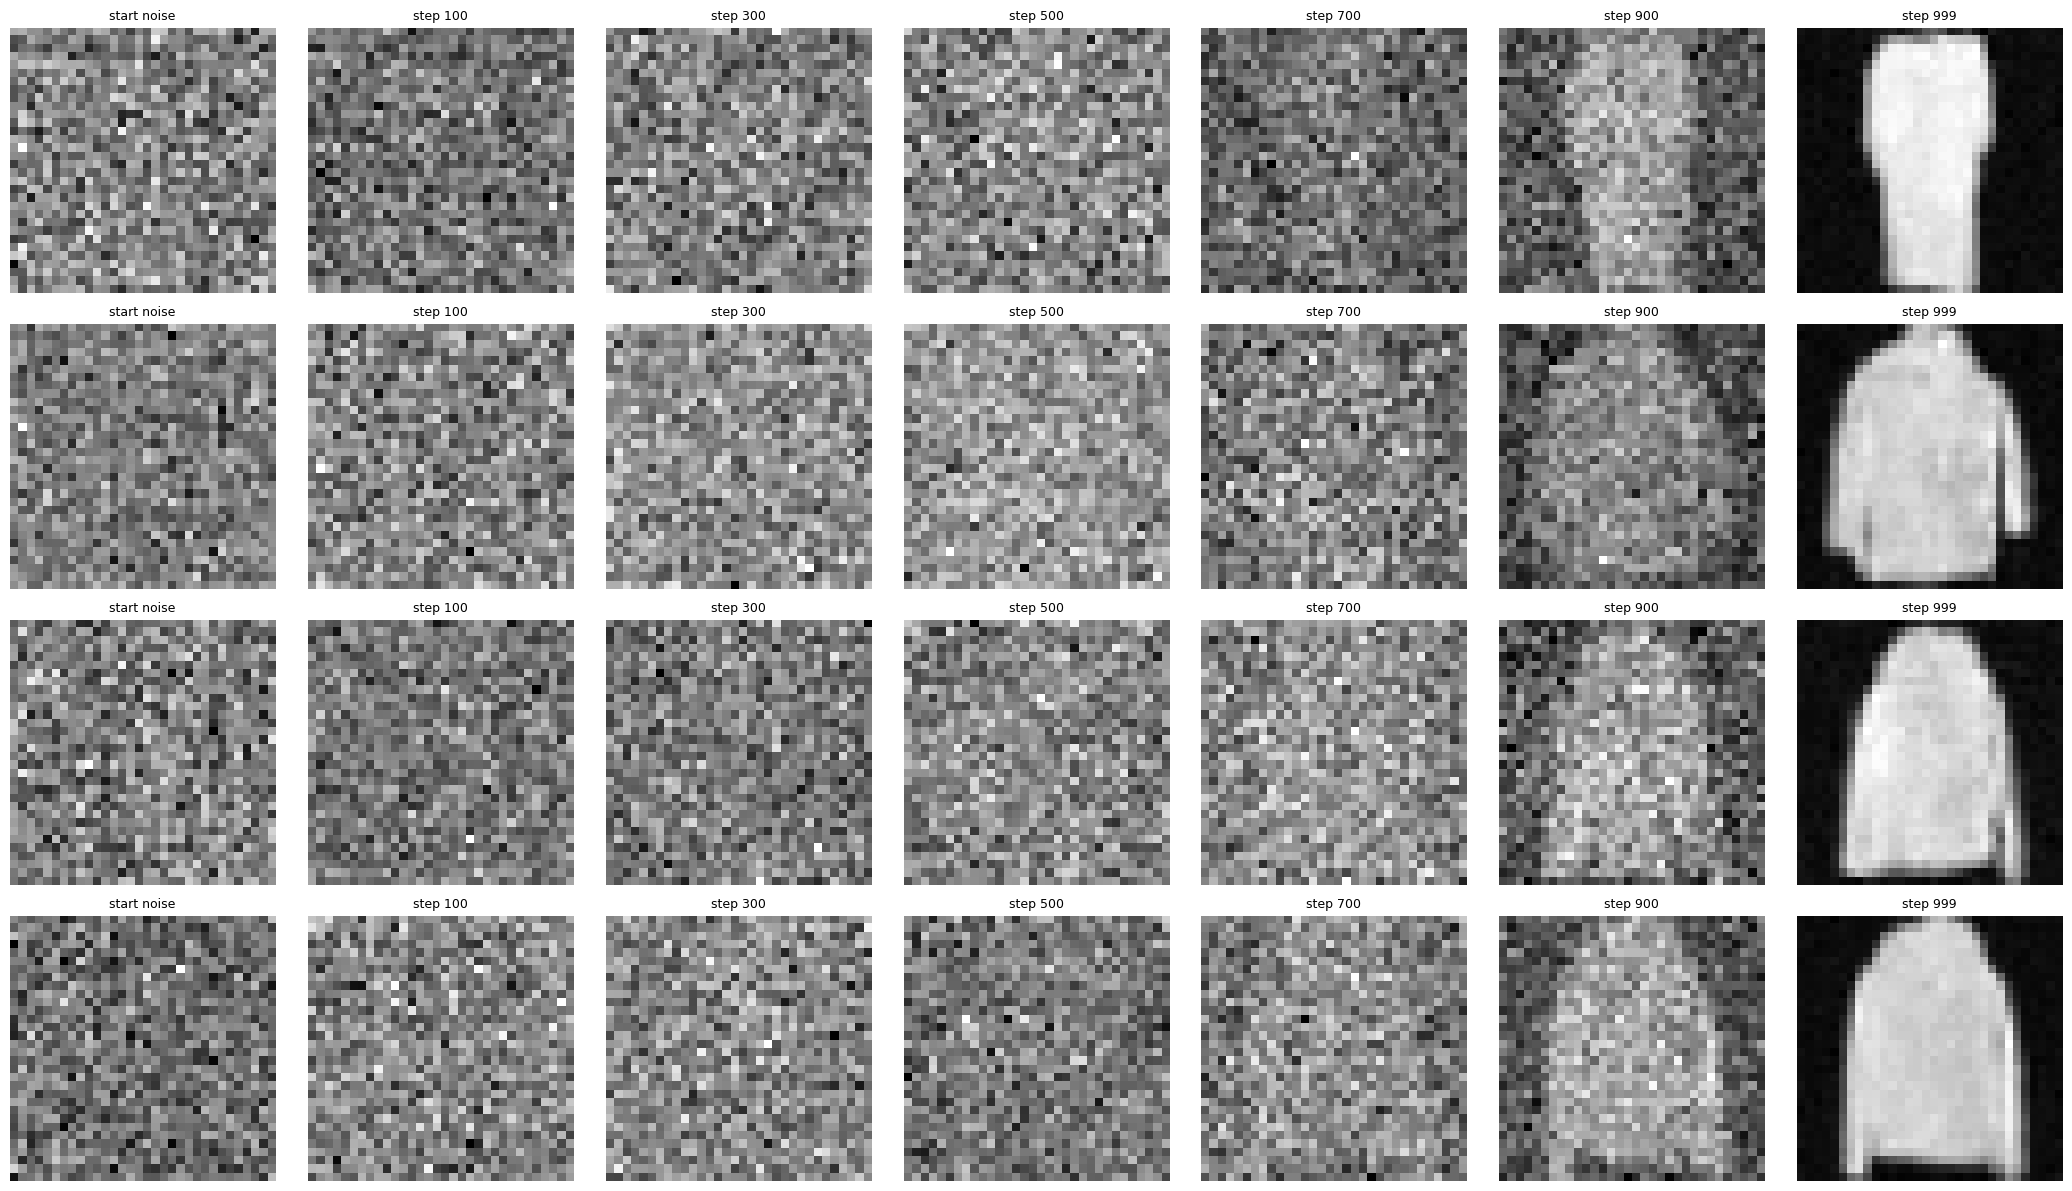
\includegraphics[width=\linewidth]{nb_q1_intermediate_denoising.png}
  \caption{Four reverse trajectories, captured at the same six points along the
           1000-step reverse chain. All four runs use the same trained network.}
  \label{fig:ddpm_intermediate}
\end{figure}

% \subsubsection*{What the earliest reverse steps look like}

At "start noise" the iterate is pure Gaussian noise, consistent with the
prior $p(\mathbf{x}_T) = \mathcal{N}(\mathbf{0}, \mathbf{I})$ that opens the
generative process, and with the iterative-denoising trajectory
$\mathbf{x}_T \to \cdots \to \mathbf{x}_0$. Through the first $\sim$700
reverse steps, the panels at step 100, 300, 500, and 700 are visually
almost indistinguishable from the starting noise. The signal weight
$\sqrt{\bar\alpha_t}$ in the forward marginal is essentially zero under the
linear $\beta$ schedule at high $t$, so the signal contribution to
$\mathbf{x}_t$ is absent and the noise prediction $\epsilon_\theta(\mathbf{x}_t, t)$
is on average close to the input itself. Inside the reverse-mean update
$\mu_\theta$ from the problem statement, the noise-prediction correction
is scaled by the factor $\beta_t / \sqrt{1-\bar\alpha_t}$, which is
small early in the chain ($\sqrt{1-\bar\alpha_t} \approx 1$ and $\beta_t$
is bounded by the schedule), so the correction barely moves the iterate
and the update mostly subtracts variance without incorporating structure.
Visually, this regime is just noise that becomes slightly less energetic
per step.

% \subsubsection*{When recognizable structure begins to appear}

A silhouette becomes recognizable only around step 900. The transition is
rapid because $\sqrt{\bar\alpha_t}$ grows quickly once the steps are past
about 700, and the factor $\beta_t / \sqrt{1-\bar\alpha_t}$ grows
alongside it as $\sqrt{1-\bar\alpha_t}$ shrinks, so the noise-prediction
correction starts to dominate the update and pulls the iterate toward a
low-frequency object outline (a body, sleeves, the rough shape of a dress
or trouser leg). At this stage the high-frequency texture is still
missing, what is visible is the silhouette and broad shading. This
concentrates the phase where structure forms in a small window near
$t = 0$, which seems to be the practical reason DDPM needs roughly
$T = 1000$ steps to sample well.

% \subsubsection*{How local detail is refined near the end of the chain}

% The last $\sim$50 steps act as a near-deterministic sharpening filter. Two
% properties of the schedule cooperate in this final tail.

% \begin{itemize}
%   \item $\beta_t$ is very small, so the injected variance
%     $\sigma_t^2 = \beta_t$ shrinks to near-zero and
%     $\mathbf{x}_{t-1} \approx \mu_\theta(\mathbf{x}_t, t)$. The chain becomes
%     effectively deterministic over these steps.
%   \item $\sqrt{\bar\alpha_t}$ is close to 1, so the signal-to-noise ratio is
%     high and the noise predictor has a clean iterate to refine.
% \end{itemize}

% The network uses these final updates to fill in edges, contrast, and
% pixel-level detail. Because the stochastic noise $\sigma_t \mathbf{z}$ is
% negligible here, the sample is effectively committed well before $t = 0$ and
% the final $\sim$50 reverse steps are doing texture synthesis rather than
% sample selection.

% \subsubsection*{Connection to the DDPM reverse-process equations}

% The observations above fall out of the Gaussian reverse transition,
% $p_\theta(\mathbf{x}_{t-1} \mid \mathbf{x}_t) = \mathcal{N}\!\left(\mathbf{x}_{t-1};\, \mu_\theta(\mathbf{x}_t, t),\, \sigma_t^2 \mathbf{I}\right)$,
% with mean
% \begin{equation}
%   \mu_\theta(\mathbf{x}_t, t)
%     = \frac{1}{\sqrt{\alpha_t}}\!\left(\mathbf{x}_t
%       - \frac{\beta_t}{\sqrt{1-\bar\alpha_t}}\,\epsilon_\theta(\mathbf{x}_t, t)\right)
%   \label{eq:ddpm_mean}
% \end{equation}
% and variance $\sigma_t^2 = \beta_t$.

% \begin{itemize}
%   \item \textbf{Early steps.} When $\bar\alpha_t \approx 0$ the prefactor
%     $\beta_t/\sqrt{1-\bar\alpha_t}$ is small (since $\sqrt{1-\bar\alpha_t}
%     \approx 1$ and $\beta_t$ is bounded by the schedule), so the
%     noise-prediction correction inside $\mu_\theta$ contributes little and
%     the update is dominated by the rescaling $\mathbf{x}_t / \sqrt{\alpha_t}$
%     plus the injected noise $\sigma_t \mathbf{z}$ of order $\sqrt{\beta_t}$.
%     The mean $\mu_\theta$ stays close to $\mathbf{x}_t$ itself, which is why
%     the early panels still look like noise.
%   \item \textbf{Onset of structure.} As $\bar\alpha_t$ grows,
%     $\sqrt{1-\bar\alpha_t}$ shrinks, the coefficient
%     $\beta_t/\sqrt{1-\bar\alpha_t}$ grows, and the noise-prediction
%     correction starts to bite. The reverse mean now differs noticeably from
%     $\mathbf{x}_t$, pulling the iterate toward the data manifold along the
%     direction $\epsilon_\theta$ predicts. Low-frequency content appears
%     first because that is what crosses the noise floor first under the
%     spectral-autoregression view of slide 20 (natural images have a
%     roughly $1/f$ power spectrum, the diffusion noise is approximately
%     spectrally flat).
%   % \item \textbf{Final refinement.} At small $t$ the variance term
%   %   $\sigma_t^2 \mathbf{I}$ collapses to near-zero, so the transition
%   %   concentrates around $\mu_\theta$. Each step becomes a small deterministic
%   %   denoising correction rather than a stochastic jump, and the network uses
%   %   these updates to add the high-frequency detail that was below the noise
%   %   floor at all earlier $t$.
% \end{itemize}

The simplified $L_2$ training loss treats every $t$ identically. The
progression to fine details is therefore not an explicit objective, it is
forced by the geometry of the schedule with $\bar\alpha_t$. Near the end
of the chain the reverse-step variance $\sigma_t^2$ shrinks to near zero,
so $\mathbf{x}_{t-1} \approx \mu_\theta(\mathbf{x}_t, t)$ and the reverse
step becomes a near-deterministic refinement that adds the high-frequency
detail buried below the noise floor at earlier $t$. Most of the chain
therefore spends its budget on coarse noise removal and only the final
tail on high-frequency synthesis.


%==============================================================================
\section*{Problem 2: Flow Matching}
%==============================================================================

% -----------------------------------------------------------------------------
\subsection*{Question 6: Theoretical comparison with DDPM}

\subsubsection*{Training objectives}

Both objectives are simple $L_2$ regressions, but they regress against
different quantities on different time domains. DDPM regresses against the
injected noise $\epsilon$ on a discrete time grid $t \in \{0, \ldots, T-1\}$
with per-step weighting implicitly defined by the $\bar\alpha_t$ schedule.
Flow Matching regresses against the constant-velocity target on the
continuous interval $t \in [0, 1]$, with no schedule-dependent weighting.
The DDPM target therefore depends on the noise schedule via $\bar\alpha_t$,
while the FM target is a constant displacement along a straight path and
decoupled from any noise schedule.

\subsubsection*{Stochastic vs.\ deterministic generation}

DDPM sampling is stochastic. Each reverse transition is a Gaussian with a
fresh noise injected at every step, so two runs from the same starting
noise $\mathbf{x}_T$ already produce different samples. Flow Matching
sampling integrates the deterministic FM ODE driven by the learned
velocity field with no noise injection, so the same starting noise always
maps to the same sample. The practical consequences are that FM
trajectories are reproducible and usable by high-order solvers like
Midpoint, while DDPM needs more reverse steps to average out the
stochastic component.

\subsubsection*{U-Net usage}

The U-Net architecture is identical in both problems. The differences are
in what the network predicts, how time is presented to it, and how its
output is composed at sampling time. DDPM uses it as
$\epsilon_\theta(\mathbf{x}_t, t)$ conditioned on a discrete timestep
index, with the output interpreted as the noise component to subtract
inside the reverse mean from the problem statement. Flow Matching reuses
the same network as $\mathbf{v}_\theta(\mathbf{x}_t, t)$ on a continuous
time $t \in [0, 1]$ that is rescaled to the same integer embedding range
via $\lfloor t \cdot 1000\rfloor$, with the output used directly as a
velocity inside the Euler / Midpoint update.

% -----------------------------------------------------------------------------
\subsection*{Question 7: Sampling quality and efficiency}

% \subsubsection*{Experimental setup}

% All sampling uses the same trained Flow Matching network and a single fixed
% batch of 16 starting noises drawn once and re-used across configurations.
% Step counts are swept on the same grid as the notebook, with Euler at
% $\{2, 5, 10, 25, 50, 100\}$ steps and Midpoint at $\{5, 10, 25, 50\}$ steps.
% The DDPM baseline reuses the $T = 1000$ stochastic reverse steps of the
% iterative-denoising trajectory in Lecture 11, slide 15, with the same starting
% noise tensor. Network-evaluation count (NFE) is $n$ for an Euler run with $n$ steps
% and $2n$ for a Midpoint run, since Midpoint uses two velocity evaluations per
% step. Wall-clock times are measured on the same RTX~3060 used for training,
% with no warm-up correction.

\subsubsection*{Results}

\begin{figure}[H]
  \centering
  \begin{subfigure}[t]{0.32\textwidth}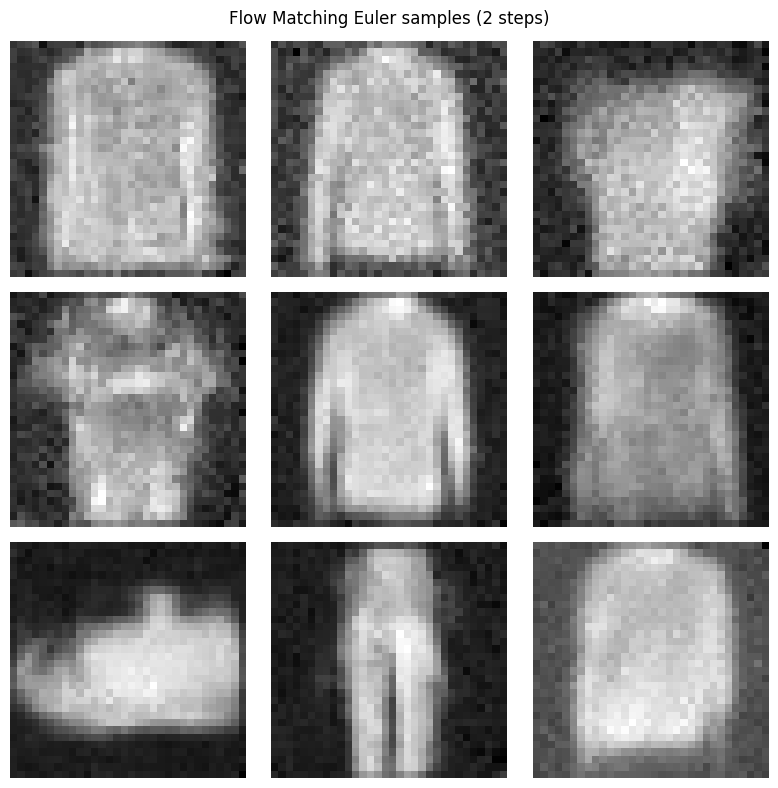
\includegraphics[width=\linewidth]{nb_q2_euler_002.png}\end{subfigure}\hfill
  \begin{subfigure}[t]{0.32\textwidth}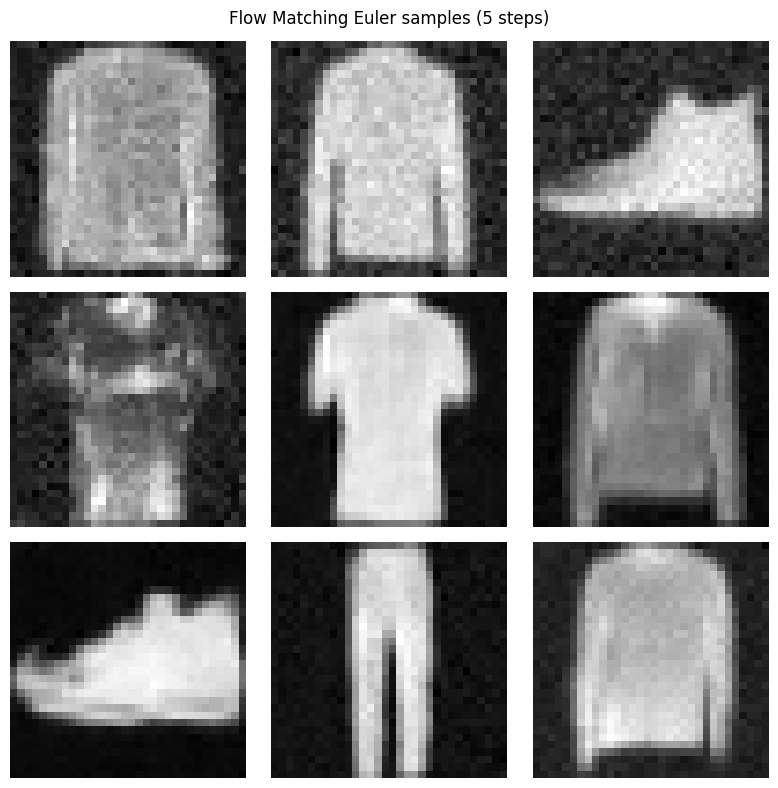
\includegraphics[width=\linewidth]{nb_q2_euler_005.png}\end{subfigure}\hfill
  \begin{subfigure}[t]{0.32\textwidth}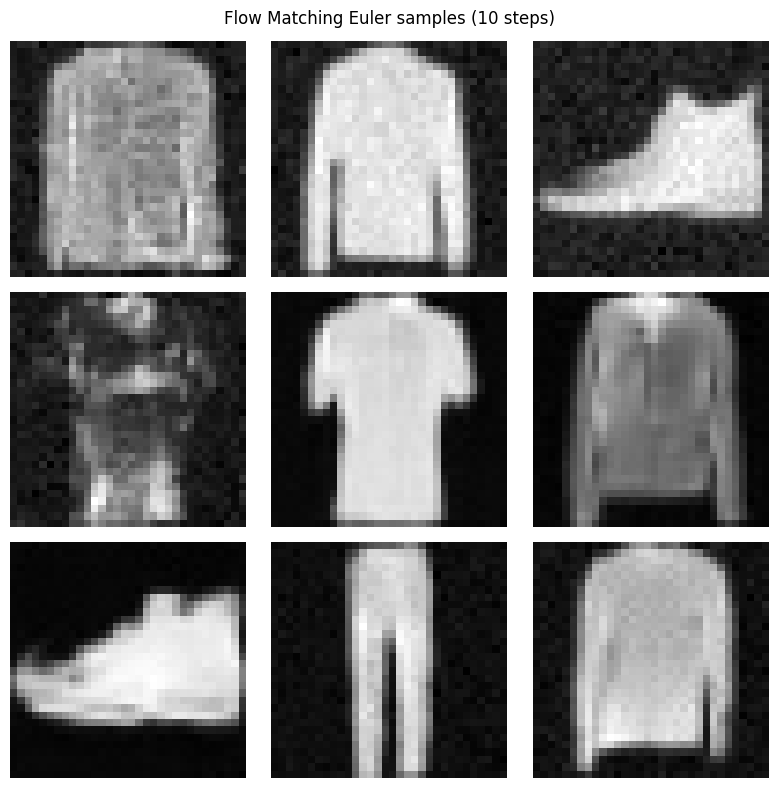
\includegraphics[width=\linewidth]{nb_q2_euler_010.png}\end{subfigure}\\
  \begin{subfigure}[t]{0.32\textwidth}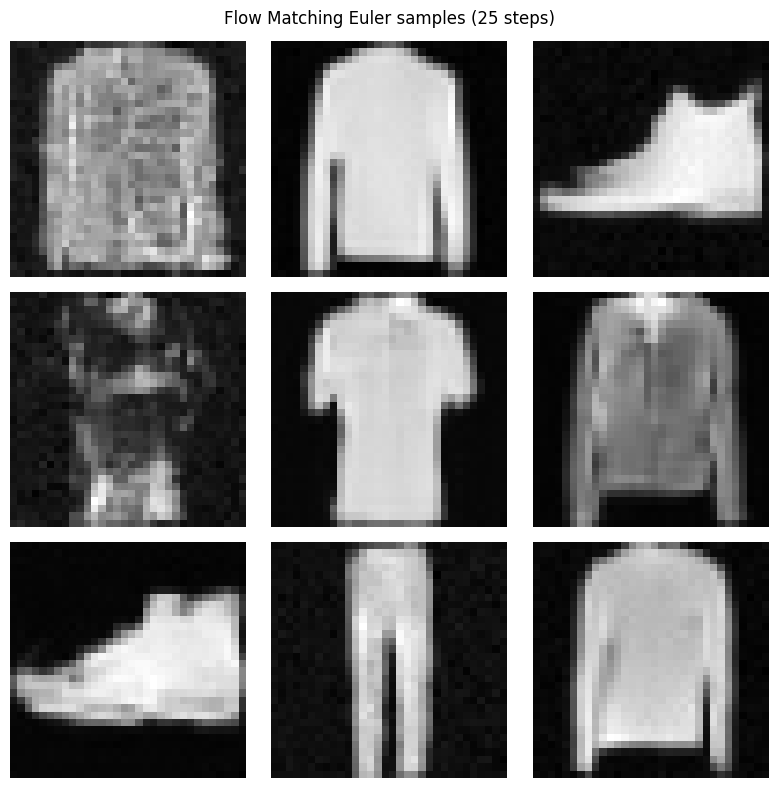
\includegraphics[width=\linewidth]{nb_q2_euler_025.png}\end{subfigure}\hfill
  \begin{subfigure}[t]{0.32\textwidth}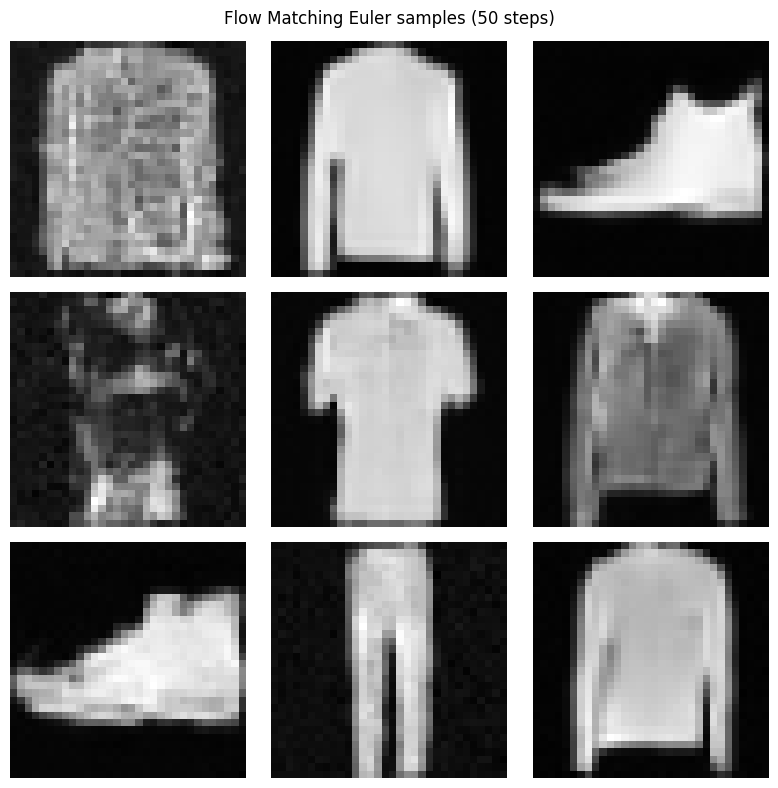
\includegraphics[width=\linewidth]{nb_q2_euler_050.png}\end{subfigure}\hfill
  \begin{subfigure}[t]{0.32\textwidth}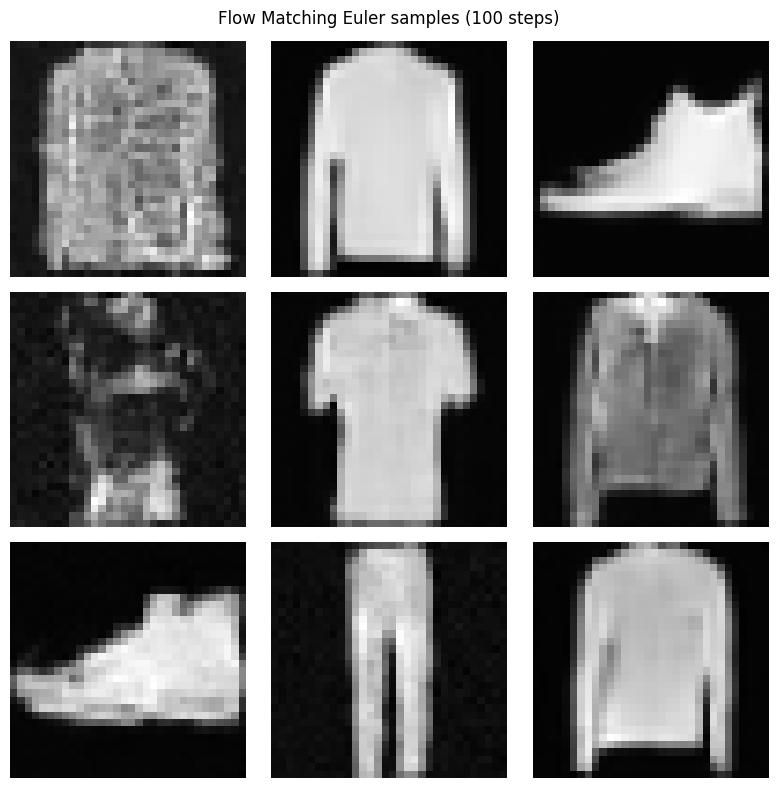
\includegraphics[width=\linewidth]{nb_q2_euler_100.png}\end{subfigure}
  \caption{Flow Matching samples under Euler integration at
           $\{2, 5, 10, 25, 50, 100\}$ steps. Each panel reuses the same fixed
           starting-noise tensor, and only the number of Euler updates changes.}
  \label{fig:fm_euler_sweep}
\end{figure}

\subsubsection*{Effect of step count on Euler}

At 2 steps Euler produces only blurry blobs with rough garment outlines but no
reliable category identity. 
Past 25 steps the marginal improvement from adding more Euler steps is
imperceptible. The 25, 50, and 100-step rows look nearly indistinguishable.
This appears to match that for a well-trained, sufficiently
smooth velocity field the Euler discretization converges fast.

\begin{figure}[H]
  \centering
  \begin{subfigure}[t]{0.40\textwidth}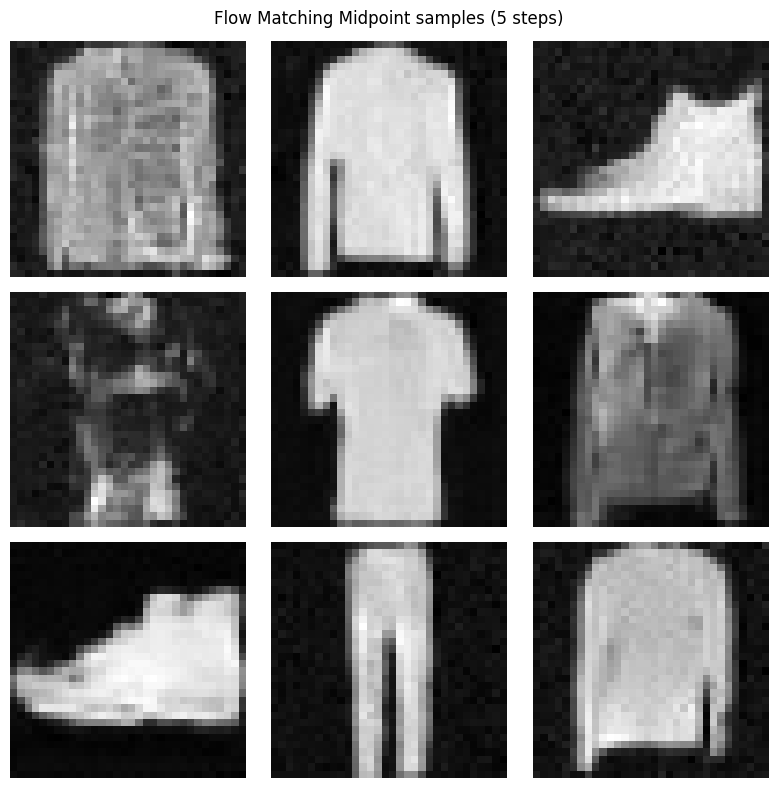
\includegraphics[width=\linewidth]{nb_q2_midpoint_005.png}\end{subfigure}\hfill
  \begin{subfigure}[t]{0.40\textwidth}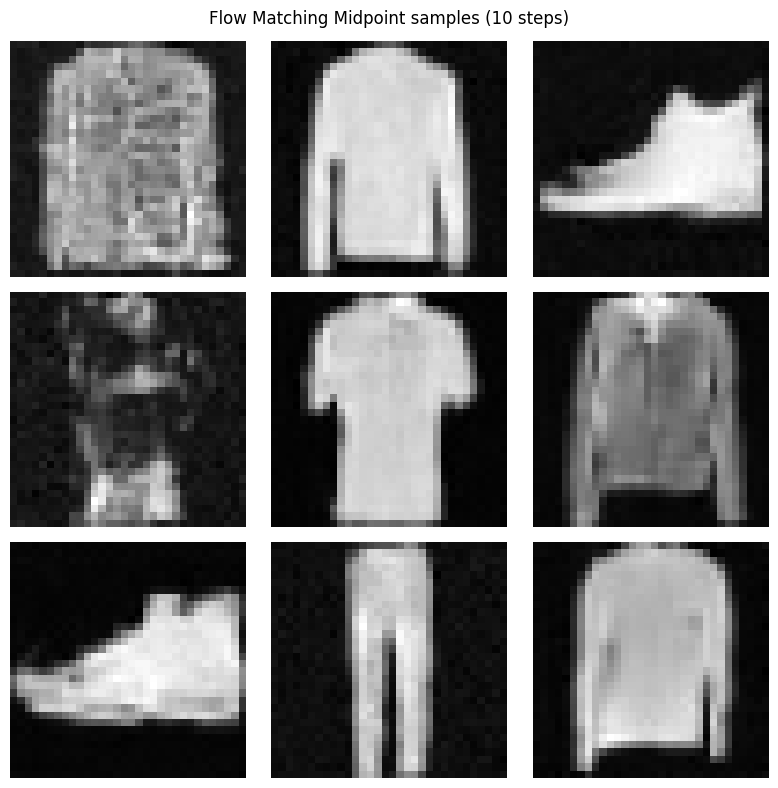
\includegraphics[width=\linewidth]{nb_q2_midpoint_010.png}\end{subfigure}\\
  \begin{subfigure}[t]{0.40\textwidth}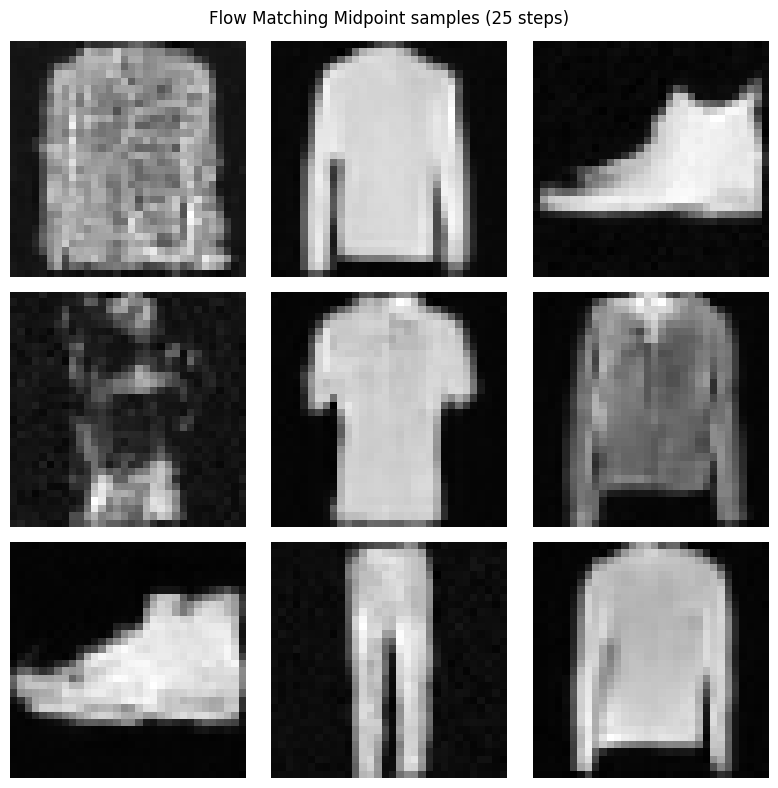
\includegraphics[width=\linewidth]{nb_q2_midpoint_025.png}\end{subfigure}\hfill
  \begin{subfigure}[t]{0.40\textwidth}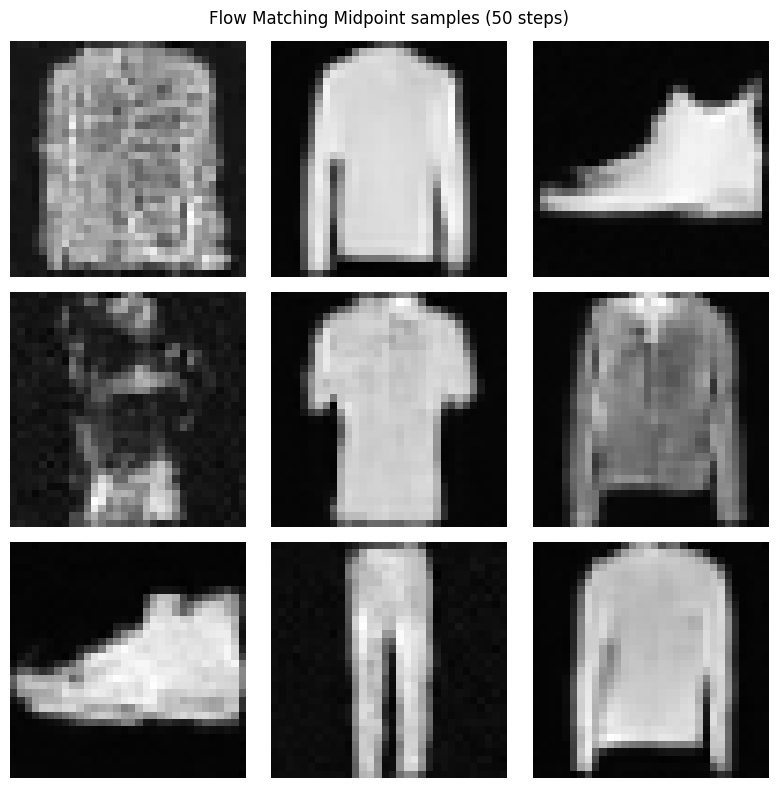
\includegraphics[width=\linewidth]{nb_q2_midpoint_050.png}\end{subfigure}
  \caption{Flow Matching samples under Midpoint integration at
           $\{5, 10, 25, 50\}$ steps. Same fixed starting noise as
           Figure~\ref{fig:fm_euler_sweep}. Midpoint uses two velocity
           evaluations per step, so the NFE budgets are $\{10, 20, 50, 100\}$.}
  \label{fig:fm_midpoint_sweep}
\end{figure}

\subsubsection*{Effect of step count on Midpoint}

Midpoint reaches usable quality much earlier. At 5 steps (NFE = 10) the samples
are already competitive with Euler at 25 steps (NFE = 25), and at 10 steps
(NFE = 20) they essentially match Euler at 100 steps. Beyond 10 steps the
Midpoint samples are also visually saturated. At matched NFE budgets, Midpoint's
second-order accuracy seems to be the deciding factor at small budgets and
becomes irrelevant at large budgets, which is the regime where a higher-order
ODE solver is expected to help.

\subsubsection*{Comparison with DDPM at matched starting noise}

\begin{figure}[H]
  \centering
  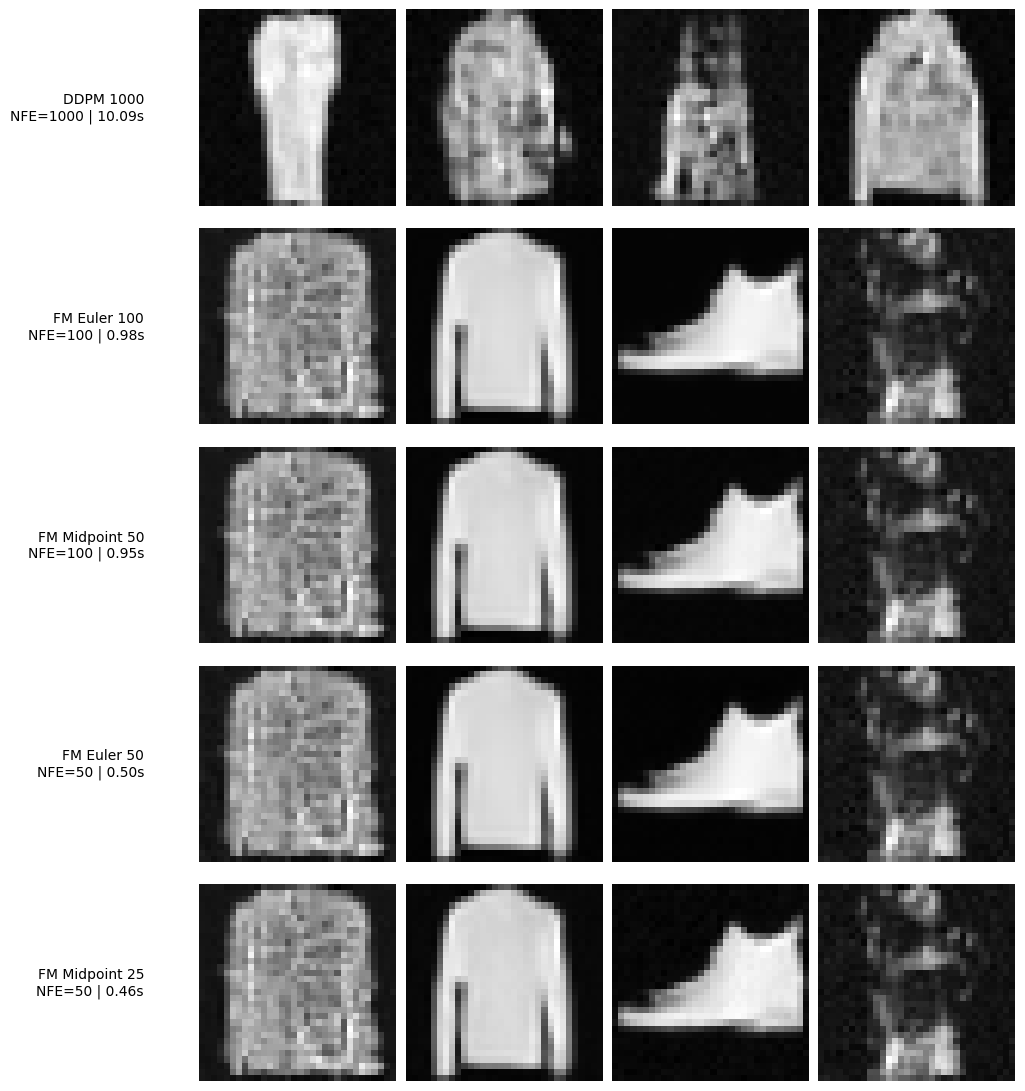
\includegraphics[width=0.85\linewidth]{nb_q2_ddpm_vs_fm.png}
  \caption{DDPM (1000-step stochastic reverse chain) compared with Flow Matching
           at four (sampler, step count) configurations. All five configurations
           use the same starting noise tensor. The per-row label reports the
           sampler, step count, NFE, and wall-clock runtime on an RTX~3060.}
  \label{fig:fm_vs_ddpm}
\end{figure}

\begin{table}[H]
  \centering
  \caption{Network-evaluation budgets and runtimes for
           Figure~\ref{fig:fm_vs_ddpm}. Wall-clock scales linearly with NFE
           within FM, and runtime is dominated by the U-Net forward pass, so
           the Midpoint and Euler runs at matched NFE finish in essentially
           identical time.}
  \label{tab:fm_runtime}
  \begin{tabular}{lrrr}
    \toprule
    Configuration       & Steps & NFE   & Runtime (s) \\
    \midrule
    DDPM (1000 steps)   & 1000  & 1000  & 10.09 \\
    FM Euler 100        &  100  &  100  &  0.98 \\
    FM Midpoint 50      &   50  &  100  &  0.95 \\
    FM Euler 50         &   50  &   50  &  0.50 \\
    FM Midpoint 25      &   25  &   50  &  0.46 \\
    \bottomrule
  \end{tabular}
\end{table}

Even with the same starting noise tensor, DDPM and FM produce visibly different
samples (Figure~\ref{fig:fm_vs_ddpm}, column-by-column). This is the expected
consequence of the stochastic-versus-deterministic distinction discussed in
Question~6, since DDPM and FM use the same starting noise for entirely
different roles (the prior $\mathbf{x}_T$ of a noisy Markov chain on one side,
and the boundary condition $\mathbf{x}_1$ of a deterministic ODE on the other).

Within the FM rows the four sampler configurations produce nearly identical
samples, which suggests both that the trained velocity field is converged and
that NFE = 50 with Midpoint is already on the plateau.

\subsubsection*{Runtime / NFE tradeoff}

Table~\ref{tab:fm_runtime} makes the practical tradeoff explicit. At equal
sample quality (DDPM vs.\ FM Midpoint 50), Flow Matching is roughly
$10.6\times$ faster in wall-clock and uses $10\times$ fewer network evaluations.
At matched NFE budgets (Euler 100 vs.\ Midpoint 50, or Euler 50 vs.\ Midpoint
25), the two FM samplers are within a few hundredths of a second of each other.
Runtime is essentially a function of NFE alone, but Midpoint's second-order
accuracy lets it use half as many integration steps. The cheapest configuration
that still produces clean samples here is FM Midpoint 25 (NFE = 50) at 0.46~s,
roughly a $22\times$ speedup over the 1000-step DDPM baseline at
indistinguishable visual quality.

\subsubsection*{Trajectory comparison with DDPM}

\begin{figure}[H]
  \centering
  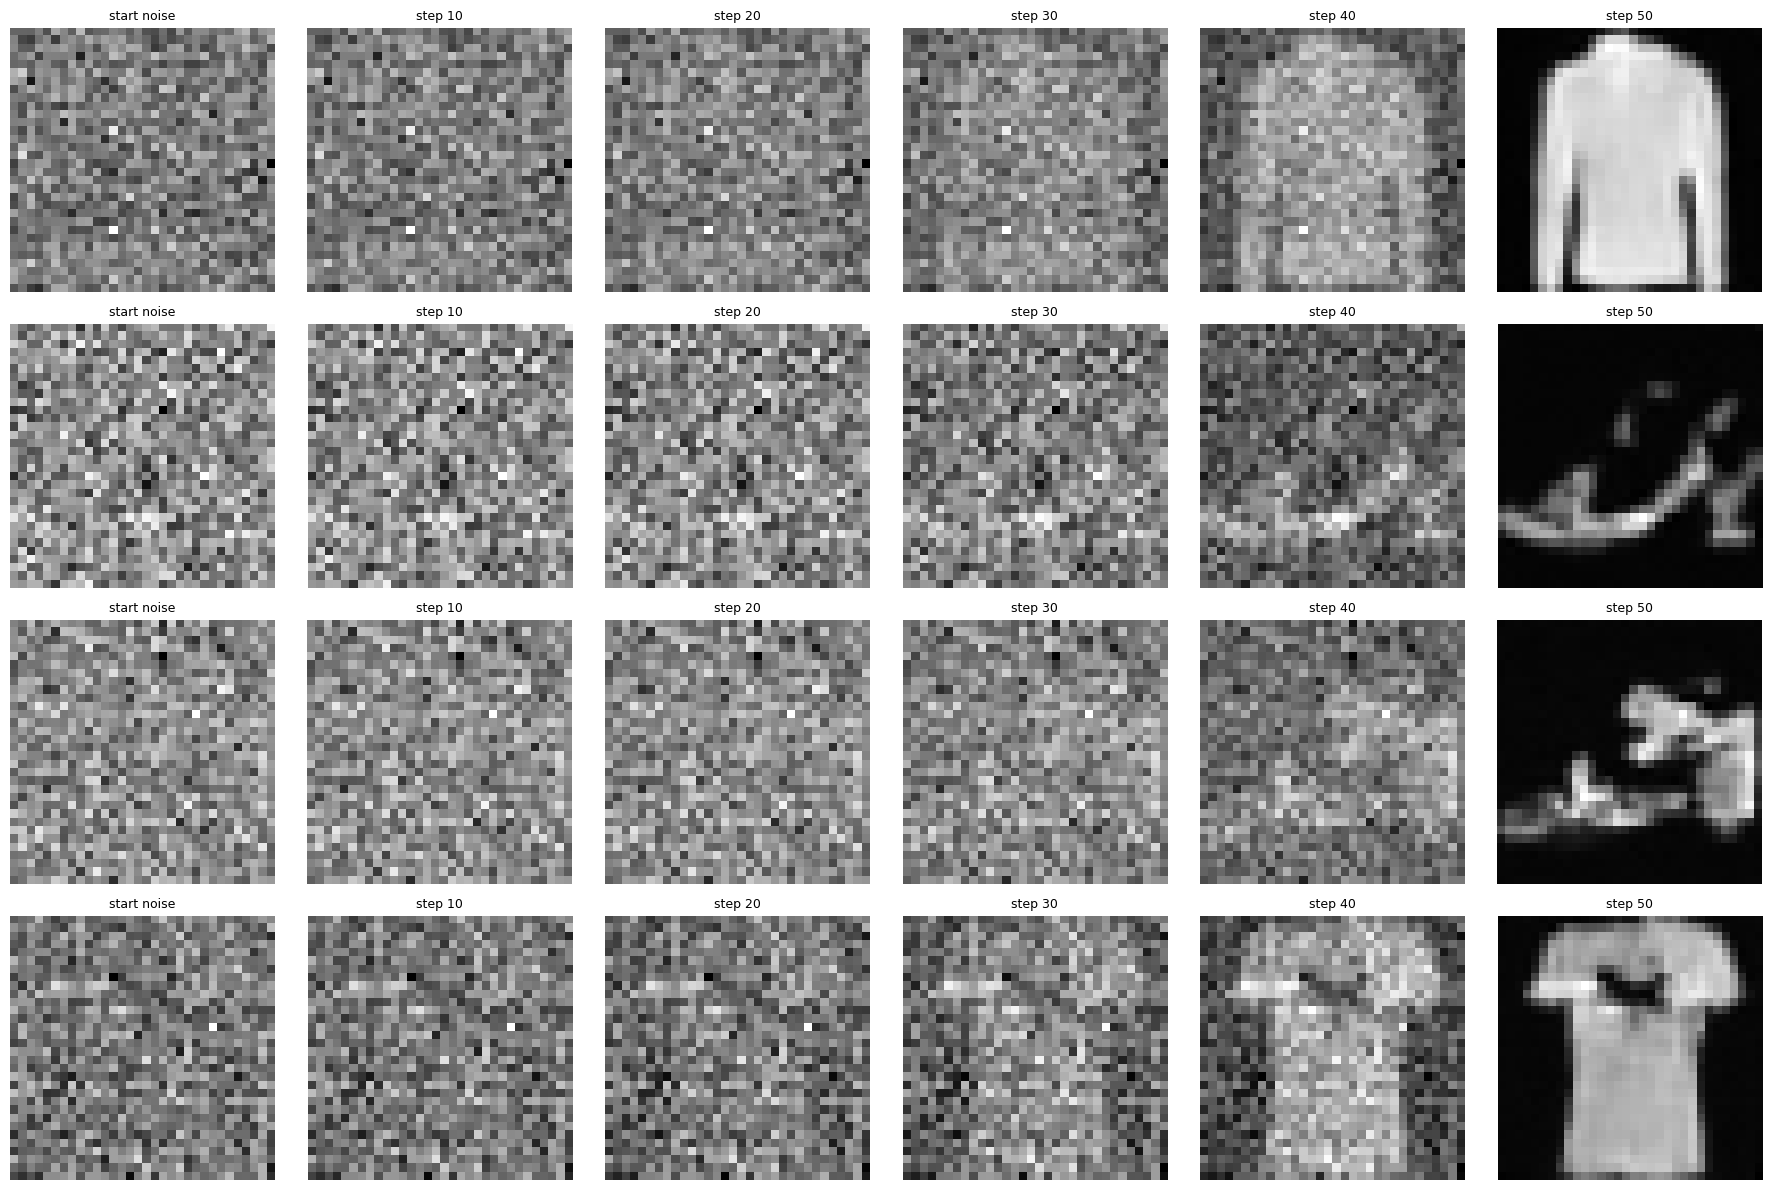
\includegraphics[width=\linewidth]{nb_q2_trajectory.png}
  \caption{Flow Matching ODE trajectory under Midpoint with 50 steps. Column
           labels record the number of completed integration steps from $t = 1$
           towards $t = 0$.}
  \label{fig:fm_trajectory}
\end{figure}

The FM trajectory in Figure~\ref{fig:fm_trajectory} mirrors the qualitative
behaviour seen for DDPM in Figure~\ref{fig:ddpm_intermediate}. The iterate
looks like noise for most of the chain and snaps to a recognizable garment
only over the last 10--20\% of the integration. The mechanism is different, but the practical
implication seems similar, with the structure-forming phase concentrated near
the data endpoint of the path.


%==============================================================================
\section*{Problem 3: Language Model Alignment}
%==============================================================================

% -----------------------------------------------------------------------------
\subsection*{Training summary}

\begin{figure}[H]
  \centering
  \begin{subfigure}[t]{0.99\linewidth}
    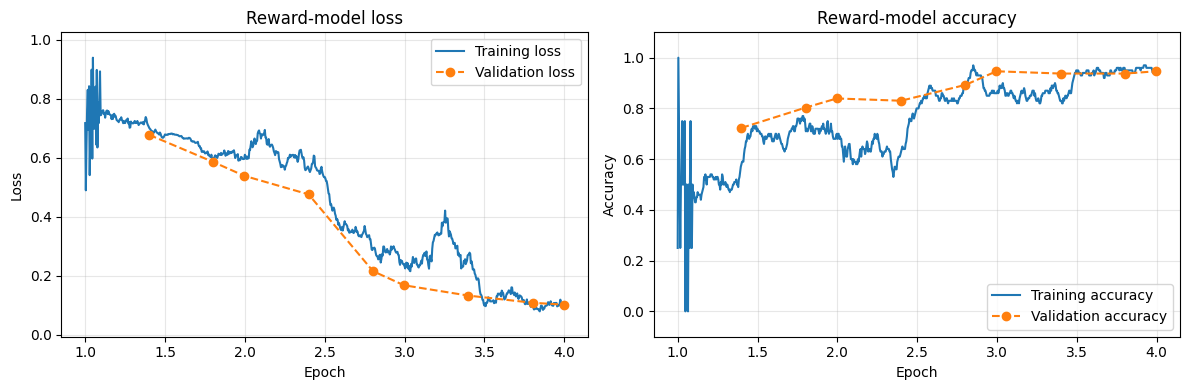
\includegraphics[width=\linewidth]{nb_q3_rm_history.png}
    \caption{Reward-model training, showing Bradley--Terry loss and pairwise accuracy.}
    \label{fig:rm_history}
  \end{subfigure}\\[0.5em]
  \begin{subfigure}[t]{0.99\linewidth}
    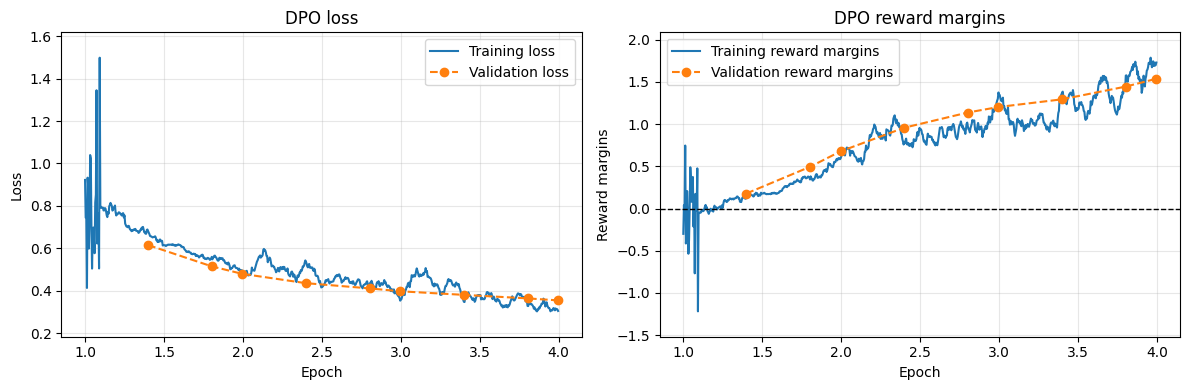
\includegraphics[width=\linewidth]{nb_q3_dpo_history.png}
    \caption{DPO training, showing loss and implicit reward margin on
             chosen minus rejected.}
    \label{fig:dpo_history}
  \end{subfigure}
  \caption{Training and validation curves for Problem 3.}
  \label{fig:q3_history}
\end{figure}

Both runs converge cleanly. The reward model reaches a held-out preference
accuracy of 94.6\% (loss $0.10$), with the validation loss dropping
from $0.69$ to $0.10$ over the 3 epochs. The DPO policy
reaches a held-out preference accuracy of 91.1\% with a mean implicit
reward margin of $1.54$. The reward margin grows roughly monotonically from
$0$ to $\approx 1.54$ during DPO training, which suggests that the policy is
consistently assigning higher likelihood than the reference to chosen
responses.

% -----------------------------------------------------------------------------
\subsection*{Question 9: DPO vs PPO theoretical comparison}

\subsubsection*{Optimizing directly from preference pairs}

PPO-based RLHF first fits an external reward model $r_\phi$ from the
preference data, then optimizes the policy with on-policy reinforcement
learning against $r_\phi$ subject to a KL penalty to $\pi_\text{ref}$.
The explicit objective is
\begin{equation*}
  \max_\pi \mathbb{E}_{\mathbf{y}\sim\pi}\!\left[r(\mathbf{x},\mathbf{y})\right]
    - \beta\,\mathrm{KL}\bigl(\pi(\cdot\mid\mathbf{x})\,\|\,\pi_\text{ref}(\cdot\mid\mathbf{x})\bigr).
\end{equation*}
DPO derives a single supervised loss on offline preference pairs that is
equivalent to optimizing this objective at the optimum. First, setting the Lagrangian's functional
derivative to zero and enforcing the normalization constraint
$\sum_\mathbf{y} \pi(\mathbf{y}\mid\mathbf{x}) = 1$ gives the policy
\begin{equation*}
  \pi^\star(\mathbf{y}\mid\mathbf{x})
    = \frac{1}{Z(\mathbf{x})}\,\pi_\text{ref}(\mathbf{y}\mid\mathbf{x})\,
      \exp\!\left(\tfrac{1}{\beta}\,r(\mathbf{x},\mathbf{y})\right),
\end{equation*}
with prompt-conditioned function
$Z(\mathbf{x}) = \sum_{\mathbf{y}}\pi_\text{ref}(\mathbf{y}\mid\mathbf{x})\,\exp(r(\mathbf{x},\mathbf{y})/\beta)$.

Taking
the log of the closed form and rearranging to express the reward in terms of the policy,
\begin{equation*}
  r(\mathbf{x},\mathbf{y}) =
    \beta\,\log\!\frac{\pi^\star(\mathbf{y}\mid\mathbf{x})}{\pi_\text{ref}(\mathbf{y}\mid\mathbf{x})}
    + \beta\,\log Z(\mathbf{x}).
\end{equation*}

Plugging this expression for
$r$ into Bradley-Terry expression yields
\begin{equation*}
  P(\mathbf{y}_w \succ \mathbf{y}_l \mid \mathbf{x}) =
    \sigma\!\left(
      \beta\,\log\!\frac{\pi^\star(\mathbf{y}_w\mid\mathbf{x})}{\pi_\text{ref}(\mathbf{y}_w\mid\mathbf{x})}
      - \beta\,\log\!\frac{\pi^\star(\mathbf{y}_l\mid\mathbf{x})}{\pi_\text{ref}(\mathbf{y}_l\mid\mathbf{x})}
    \right),
\end{equation*}
since the $\beta\log Z(\mathbf{x})$ terms cancel in the difference.

Treating the unknown optimum
$\pi^\star$ as a trainable policy $\pi_\theta$, the negative log-likelihood
of the observed preference pairs is exactly the DPO loss from the problem
statement,
\begin{equation}
  \mathcal{L}_\text{DPO} =
    -\mathbb{E}_{(\mathbf{x},\mathbf{y}_w,\mathbf{y}_l)}\!\left[
      \log \sigma\!\left(
        \beta\!\left(
          \log\!\frac{\pi_\theta(\mathbf{y}_w\mid\mathbf{x})}{\pi_\text{ref}(\mathbf{y}_w\mid\mathbf{x})}
          - \log\!\frac{\pi_\theta(\mathbf{y}_l\mid\mathbf{x})}{\pi_\text{ref}(\mathbf{y}_l\mid\mathbf{x})}
        \right)
      \right)
    \right].
  \label{eq:dpo}
\end{equation}
The result is a binary cross-entropy on the reward between the chosen and rejected responses, so it can be optimized
with ordinary backpropagation on offline pairs. The gradient at each pair pushes
$\log\pi_\theta(\mathbf{y}_w)$ up and $\log\pi_\theta(\mathbf{y}_l)$ down, so updates are large for pairs
the policy currently ranks incorrectly and small for pairs already correctly
ranked. There is no rollout policy, no on-policy sampling, and no separately
trained $r_\phi$, and so it optimizes effectively from preference pairs only.

\subsubsection*{Role of the frozen reference model and the limit $\beta \to 0$}

The reference model $\pi_\text{ref}$ acts as an anchor for the policy.
In Equation~\ref{eq:dpo}, $\pi_\text{ref}$ only appears inside the
log-ratios $\log[\pi_\theta(\mathbf{y})/\pi_\text{ref}(\mathbf{y})]$ that
sit inside $\sigma$, so the DPO loss only registers deviations of
the policy from the reference rather than absolute likelihoods. The
coefficient $\beta$ multiplies the entire log-ratio difference inside
$\sigma$ and sets how strict that anchor is. Larger $\beta$ keeps the
policy close to the reference and slows learning. Smaller $\beta$ relaxes
the anchor and lets the policy move further per step.

If $\beta \to 0$ (or the reference is removed entirely), the anchor
disappears. Equation~\ref{eq:dpo} is then minimized only by sending the
log-ratio margin between chosen and rejected responses to $+\infty$, with
nothing pulling the policy back toward $\pi_\text{ref}$. The policy can
pile arbitrarily large probability on the chosen responses and
arbitrarily little on the rejected ones. In practice this means the policy loses the
natural writing style it picked up during SFT, any mistakes the human
labelers made get amplified instead of smoothed out, and the policy
starts picking up on accidental patterns in the training pairs rather
than on what the labelers actually cared about (reward hacking). PPO controls it with an explicit KL penalty, and
DPO bakes the same effect into its loss through the log-ratio.

\subsubsection*{Advantage and disadvantage relative to PPO}

\paragraph{Advantage:} DPO is simpler to set up and run than PPO. It
trains one model with a regular supervised loss on a fixed dataset of
preference pairs. PPO instead needs a separately trained reward model, a
loop that generates and scores fresh responses during training, and a
value network to estimate baselines for the RL update. With fewer moving
parts, DPO has just one main hyperparameter ($\beta$) to tune instead of
the many PPO needs, which makes it more stable and easier to
reproduce across runs.

\paragraph{Disadvantage:} DPO can only learn from the preference pairs it
sees during training. Once those are fixed, it has no way of asking the
reward signal about new responses, so prompts or response styles outside
the training data get no useful update. PPO does not have this problem
because it keeps generating fresh candidates from the current policy at
each step and scoring them with the reward model, which lets it correct
itself on responses the static dataset never contained. Iterative DPO, we have seen, closes most of the gap by periodically re-sampling
preference pairs from the current policy, recovering the on-policy
property of PPO without the RL part.

% -----------------------------------------------------------------------------
\subsection*{Question 10: Best-of-$N$ analysis}

\subsubsection*{Mean reward as a function of $N$}

\begin{figure}[H]
  \centering
  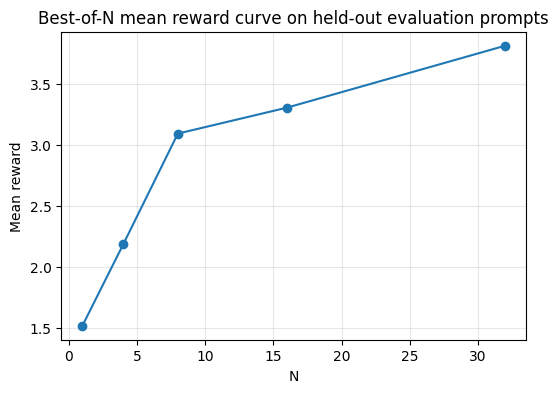
\includegraphics[width=0.55\linewidth]{nb_q3_bon_curve.png}
  \caption{Best-of-$N$ mean reward over 5 held-out evaluation prompts,
           $N \in \{1, 4, 8, 16, 32\}$.
           The curve is monotone and concave in $N$ with diminishing returns
           past $N\!\approx\!16$.}
  \label{fig:bon_curve}
\end{figure}

From figure~\ref{fig:bon_curve}, the mean reward of the Best-of-$N$
selection on the held-out prompts grows monotonically with $N$, from $\approx 1.5$ at $N=1$ to
$\approx 3.8$ at $N=32$. The steepest gain is between $N=1$ and $N=8$
($\approx +1.6$), and there are clearly diminishing returns past $N=16$.

The shape of the curve is what one would expect from picking the maximum
out of a larger and larger pool of candidates. Doubling $N$ doubles the
chances of hitting an unusually good candidate, but the gain shrinks fast
because most of the easy improvement comes from avoiding the worst few
candidates and the rest is rarer luck. Doubling $N$ from 16 to 32 only
buys about $+0.5$ reward at twice the inference cost.

\subsubsection*{Best-of-1 vs.\ Best-of-16 on a held-out prompt}

For the prompt \emph{"Explain what a sonnet is."}, the same DPO policy produces these two candidates.

\begin{itemize}
  \item \textbf{Best-of-1} (reward $3.78$): \emph{"A sonnet is a type of
    poetic composition in which the primary subject is a child or child-like
    figure. It typically begins with the words 'I am' or 'I sing.'\,"}
  \item \textbf{Best-of-16} (reward $6.37$): \emph{"A sonnet is a piece of
    music composed for the sole purpose of expressing an idea. It typically
    begins with a strong, melodic voice, which typically changes to a more
    verse or a more lyrical voice, typically in the second or"}
\end{itemize}

\subsubsection*{Does higher reward match human judgment?}

Not on this prompt. A sonnet is a 14-line poem with a fixed rhyme scheme.
Both candidates are factually wrong, and the Best-of-16 answer is arguably
worse. It asserts that a sonnet is "a piece of music" rather than a
poem, and trails off mid-sentence at the 128-token cap. Yet it scores nearly
twice as high as Best-of-1.

The reward model is just an approximation of what a human would prefer.
As $N$ grows, Best-of-$N$ searches harder and harder for the candidate
that the reward model rates highest, which is not the same thing as the
candidate a human would actually prefer. This is a reward hacking
failure, where optimizing a proxy hard enough makes its score go up while
the true quality stagnates or even goes down. A few specific
reward-model limitations show up here:

\begin{itemize}
  \item The reward model seems to prefer longer
    responses with a confident, instruction-tuned tone even when they
    are factually wrong.
  \item The reward model is a small
    GPT-2 fine-tuned on about a thousand preference pairs and is never told
    what is actually true about the world, so it cannot really tell a
    correct definition apart from a confident-sounding wrong one.
  \item Literary definitions are probably
    underrepresented in this small training set, so on a prompt about
    sonnets the reward model has nothing solid to fall back on and just
    picks whichever surface form looks the most polished.
\end{itemize}

The practical takeaway is that Best-of-$N$ amplifies whatever biases the
reward model already has. The quality ceiling is set by the reward model
itself, and on prompts where the reward model is unreliable, larger $N$
can actively make things worse.

\end{document}
